\section{Mathematical Toolkit}
\label{app:toolkit}
This companion collects the background facts used in the main-text proofs.
All random vectors in the projection statements are square-integrable, and
all weighting matrices $Q$ are deterministic and positive definite.

\subsection{Information as \texorpdfstring{$\sigma$}{sigma}-algebras}
\label{app:toolkit-1}
\textbf{$\sigma$-algebra generated by a variable.} For a random vector $Y$, $\sigma(Y)$ is the collection of all events whose occurrence can be decided by looking at $Y$. It formalizes "what is known if one observes $Y$."

\textbf{Measurability means "a function of".} By the Doob--Dynkin lemma, a random variable $u$ is $\sigma(Y)$-measurable if and only if $u=g(Y)$ for some (measurable) function $g$. So "$u_i$ is $\mathcal G_i$-measurable" means "$u_i$ is computed from agent $i$'s observations."

\textbf{Combining information.} $\sigma(Y)\vee\sigma(Z)=\sigma(Y,Z)$ is the information from observing both.

\textbf{Nesting.} $\mathcal G\subseteq\mathcal G'$ means that whoever knows $\mathcal G'$ knows at least everything in $\mathcal G$. Every $\mathcal G$-measurable rule is then also $\mathcal G'$-measurable.

\subsection{Geometry of square-integrable random vectors}
\label{app:toolkit-2}
\textbf{The space $L^2$.} Random vectors $u$ with $\mathbb E\|u\|^2<\infty$, with inner product $\langle u,v\rangle_Q=\mathbb E[u^\top Qv]$ for a fixed positive-definite $Q$. This is a Hilbert space: an inner-product space in which limits of Cauchy sequences stay in the space.

\textbf{Projection theorem.} For a closed linear subspace $S$ and any $x$, there is a unique $\Pi x\in S$ closest to $x$. It is characterized by orthogonality: $\langle x-\Pi x,\,s\rangle_Q=0$ for all $s\in S$.

\textbf{Pythagoras.} $\|x\|^2=\|\Pi x\|^2+\|x-\Pi x\|^2$. More generally, for any $s\in S$, $\|x-s\|^2=\|x-\Pi x\|^2+\|\Pi x-s\|^2$.

\textbf{Conditional expectation is a projection.} $\mathbb E[x\mid\mathcal G]$ is the orthogonal projection of $x$ onto $\{\mathcal G\text{-measurable }L^2\text{ variables}\}$. It is therefore the best mean-square predictor of $x$ among \emph{all} functions of the information, not only linear ones.

\textbf{Tower property.} For square-integrable $g(Y)$ and $Z$, $\mathbb E[g(Y)^\top Z]=\mathbb E\big[g(Y)^\top\mathbb E[Z\mid Y]\big]$. \emph{Consequence:} if $\mathbb E[\varepsilon\mid Y]=0$, then $\varepsilon$ is orthogonal to every function of $Y$. This is the step used in Lemma~\ref{lem:innovation_split}.

\textbf{Common information makes the optimizer independent of $Q$.} If every component of the policy may depend on the same $\sigma$-algebra $\mathcal G$, the $Q$-projection of $x$ is simply $\mathbb E[x\mid\mathcal G]$, for any positive-definite $Q$. The error $e=x-\mathbb E[x\mid\mathcal G]$ satisfies $\mathbb E[s^\top Qe]=\mathbb E\big[s^\top Q\,\mathbb E[e\mid\mathcal G]\big]=0$ for every $\mathcal G$-measurable $s$. With \emph{different} information per agent, this fails and the coupled equations \eqref{eq:block_conditional_normal_equations} are needed.

\textbf{Regret and the factor one-half.} Completing the square in the main
paper's quadratic cost gives $R(\mathcal A)=\tfrac12\|x^\star-u^\star_{\mathcal A}\|_Q^2$.
Consequently a squared $Q$-norm in a proof equals twice the corresponding
regret. The best constant action is $\bar x^\star=\mathbb E[x^\star]$, since
\[
\|x^\star-c\|_Q^2=\|x^\star-\bar x^\star\|_Q^2+
(\bar x^\star-c)^\top Q(\bar x^\star-c).
\]
Thus $2R_\infty=\|x^\star-\bar x^\star\|_Q^2$.

\textbf{Mean-square convergence.} $Y_n\to Y$ in $L^2$ means $\mathbb E\|Y_n-Y\|^2\to0$.

\subsection{Gaussian facts}
\label{app:toolkit-3}
\textbf{Conditioning.} If $(X,Y)$ is jointly Gaussian and $\Sigma_{YY}$ is invertible,

\[
\mathbb E[X\mid Y]=\mu_X+\Sigma_{XY}\Sigma_{YY}^{-1}(Y-\mu_Y),\qquad \operatorname{Cov}(X\mid Y)=\Sigma_{XX}-\Sigma_{XY}\Sigma_{YY}^{-1}\Sigma_{YX}.
\]

  The conditional mean is affine in $Y$ (linear after centering). For singular
$\Sigma_{YY}$, the same formulas use its Moore--Penrose inverse on the covariance support. The conditional covariance (a \emph{Schur complement}) does \textbf{not} depend on the observed value of $Y$.

\textbf{Scalar case.} For nonzero marginal variances, $\operatorname{Var}(X\mid Y)=\operatorname{Var}(X)\big(1-\operatorname{Corr}(X,Y)^2\big)$.

\textbf{Uncorrelated implies independent} for jointly Gaussian variables. For the OU process, Brownian increments after the snapshot time are independent
of the past, which gives innovation independence in Section~\ref{app:toolkit-4}.

\textbf{Linear functionals stay Gaussian.} Integrals such as $\int w(u)\theta(u)\,du$ defined as mean-square limits of linear combinations of a Gaussian field are Gaussian, so the facts above apply to $x^\star$ in Section~\ref{subsec:canonical_line_model}.

\subsection{The Ornstein--Uhlenbeck process in time}
\label{app:toolkit-4}
\textbf{Scalar SDE.} $d\theta_t=-\tfrac1T(\theta_t-\bar\theta)\,dt+\sigma\sqrt{2/T}\,dW_t$, where $W$ is Brownian motion (continuous paths, independent Gaussian increments with variance equal to elapsed time). A useful mental model is the small-step recursion

\[
\theta_{t+\Delta}\approx\theta_t-\tfrac{\Delta}{T}(\theta_t-\bar\theta)+\sigma\sqrt{2\Delta/T}\,Z,\qquad Z\sim N(0,1)\text{ fresh at each step}.
\]

\textbf{Solution over a lag $\tau$.}

\[
\theta_t-\bar\theta=e^{-\tau/T}(\theta_{t-\tau}-\bar\theta)+\underbrace{\sigma\sqrt{2/T}\int_{t-\tau}^{t}e^{-(t-s)/T}dW_s}_{\varepsilon_{t,\tau}} .
\]

  The innovation is Gaussian with mean zero, independent of the past, and has variance $\sigma^2\tfrac2T\int_0^\tau e^{-2s/T}ds=\sigma^2(1-e^{-2\tau/T})$. This shows why the factor $\sqrt{2/T}$ makes the stationary variance equal $\sigma^2$.

\textbf{Correlation.} In stationarity, $\operatorname{Corr}(\theta_t,\theta_s)=e^{-|t-s|/T}$. The coherence time $T$ is the lag at which correlation falls to $1/e\approx0.37$.

\textbf{Multivariate, common rate \eqref{eq:OU_process}.} Replace $\sigma$ by $\Sigma_\infty^{1/2}$, the symmetric positive-semidefinite matrix whose square is $\Sigma_\infty$. Every formula above holds with $\sigma^2$ replaced by $\Sigma_\infty$, because the drift $-\tfrac1T I$ treats all directions alike.

\textbf{Markov property.} The future after time $s$ depends on the past only through $\theta_s$.

\textbf{Discrete-time analogue.} AR(1): $\theta_k-\bar\theta=a(\theta_{k-1}-\bar\theta)+\varepsilon_k$. In its stationary solution with $|a|<1$ and i.i.d. square-integrable
innovations independent of the past, each nondegenerate scalar component
has correlation $a^{|h|}$ at lag $h$.

\subsection{Exponential covariance in space; fields on graphs}
\label{app:toolkit-5}
\textbf{1-D spatial OU.} A Gaussian field on the line with covariance $\sigma^2e^{-|z-z'|/\ell_s}$ is an OU process in the spatial coordinate. It is Markov in $z$: given $\theta(z_0)$, the field on either side of $z_0$ is conditionally independent of the other side. Given a whole segment, the outside depends only on the nearer endpoint.

\textbf{Gaussian Markov random fields (GMRFs).} On an undirected graph, a Gaussian vector with nonsingular covariance is Markov with respect to the graph when each node, given its neighbors, is independent of all other nodes. Equivalently, the precision matrix $\Sigma^{-1}$ has zeros for non-adjacent pairs.

\textbf{Graph Laplacian.} $L_G=D_G-A_G$, where $D_G$ is the diagonal degree matrix and $A_G$ the adjacency
matrix of a simple undirected unweighted graph. For a signal $x$, $x^\top L_Gx=\sum_{(i,j)\in E}(x_i-x_j)^2$ measures roughness. Eigenvectors of $L_G$ with small eigenvalues ("low graph frequencies") vary slowly across edges.

\textbf{Covariance \eqref{eq:graph_spectral_covariance}.} $\Sigma_S=\sigma^2(\kappa_s^2I+L_G)^{-\nu}$ puts large variance on low-frequency (smooth) patterns. After normalizing total variance, smaller $\kappa_s$ or larger $\nu$ shifts
relative energy toward smoother modes. This spectral model need not have a
sparse precision matrix for arbitrary $\nu$, so it need not be Markov on
the original graph.

\subsection{Matrix facts}
\label{app:toolkit-6}
\textbf{Quadratic-form expectation.} For a random vector $Y$ with mean $\mu$, $\mathbb E[Y^\top AY]=\operatorname{tr}(A\operatorname{Cov}Y)+\mu^\top A\mu$.

\textbf{Cyclic trace.} $\operatorname{tr}(ABC)=\operatorname{tr}(BCA)=\operatorname{tr}(CAB)$ whenever the products are defined.

\textbf{Sherman--Morrison.} For invertible $A$ and vectors $a,c$ with $1+c^\top A^{-1}a\neq0$,

\[
(A+ac^\top)^{-1}=A^{-1}-\frac{A^{-1}ac^\top A^{-1}}{1+c^\top A^{-1}a}.
\]

  With $A=qI$ and $a=\gamma\mathbf 1$, $c=\mathbf 1$ this gives $(qI+\gamma\mathbf 1\mathbf 1^\top)^{-1}=\frac1q\big(I-\frac{\gamma}{q+\gamma n}\mathbf 1\mathbf 1^\top\big)$. Also $\operatorname{tr}(qI+\gamma\mathbf 1\mathbf 1^\top)=n(q+\gamma)$.

\textbf{Positive-definite weighting.} $Q\succ0$ means $x^\top Qx>0$ for all $x\neq0$. Then $\lambda_{\min}(Q)\|x\|^2\le x^\top Qx\le\lambda_{\max}(Q)\|x\|^2$, so the $Q$-norm and the ordinary norm are equivalent.

\textbf{Null space and modes.} The null space of $K$ is $\{\xi:K\xi=0\}$. A "mode" of the state is a direction $\xi$, often an eigenvector of $\Sigma_S$. Its decision-error weight per unit state variance is $(K\xi)^\top Q(K\xi)$.

\subsection{Calculus, asymptotics, and optimization}
\label{app:toolkit-7}
\textbf{Log-derivative.} $\frac{d}{dr}\log f(r)=f'(r)/f(r)$ is the \emph{relative} growth rate of $f$, the fractional change per unit $r$. The spatial rate $m_S$ is the log-derivative of the explained spatial share; $m_T$ is the negative log-derivative of the temporal factor $e^{-2\tau(r)/T}$.

\textbf{First-order conditions.} At an interior minimum of a differentiable function the derivative vanishes. The converse fails: a zero derivative identifies candidates only.

\textbf{Single crossing.} If $\Delta(r)$ is continuous and strictly decreasing, it has at most one zero. The function whose derivative has the sign of $-\Delta$ is then unimodal, with its minimum at that zero, or at an endpoint if there is no zero.

\textbf{Continuous relaxation.} Solving an integer problem (radius in hops) by first allowing real values. When the continuous objective is unimodal, the integer optimum is the better of the two integers bracketing the continuous optimum.

\textbf{Taylor approximations used.} $1-e^{-x}\approx x$ and $\log(1+x)\approx x$ for small $x$.

\textbf{Asymptotic notation.} $f=O(g)$ means $|f|\le C|g|$ near the limit; $f=o(g)$ means $f/g\to0$.

\textbf{Positive part and extended reals.} $[z]_+=\max\{z,0\}$. Writing $\rho^\star=+\infty$ means that no finite value satisfies the condition.

\clearpage
\section{Glossary}
\label{app:glossary}
The entries below use the meanings and assumptions of this paper.
\small
\setlength{\tabcolsep}{4pt}
\renewcommand{\arraystretch}{1.12}
\begin{longtable}{@{}p{.23\linewidth}p{.52\linewidth}p{.20\linewidth}@{}}
\toprule
Term & Meaning in this paper & First use/background \\
\midrule
\endfirsthead
\toprule
Term & Meaning in this paper & First use/background \\
\midrule
\endhead
\bottomrule
\endfoot
Information architecture & Specification of which variables, at which ages, each agent's decision may depend on; formally a tuple of $\sigma$-algebras $(\mathcal G_1,\dots,\mathcal G_n)$ & Section~\ref{subsec:architectures} \\
$\sigma$-algebra $\sigma(Y)$ & "What is known from observing $Y$" & Section~\ref{subsec:architectures}, Section~\ref{app:toolkit-1} \\
Measurable ($\mathcal G_i$-measurable) & Computable from agent $i$'s information & \eqref{eq:policy_subspace}, Section~\ref{app:toolkit-1} \\
Admissible policy & A joint rule in which each agent uses only its own information & \eqref{eq:policy_subspace} \\
Static team & Several decision makers with one shared objective, each acting on its own information, whose actions do not affect anyone's later information & Section~\ref{sec:introduction}, Section~\ref{subsec:related_static} \\
Person-by-person (stationarity) conditions & Each agent's rule is optimal given the others' rules; here, equations \eqref{eq:conditional_normal_equations}--\eqref{eq:block_conditional_normal_equations} & Corollary~\ref{cor:conditional_normal_equations} \\
Full-information (clairvoyant) decision & $x^\star_t=Q^{-1}b(\theta_t)$, optimal with complete current state & \eqref{eq:clairvoyant} \\
Architecture regret & Extra expected cost versus the full-information decision, after optimizing over admissible policies & \eqref{eq:architecture_regret} \\
$Q$-weighted norm & $\|u\|_Q^2=\mathbb E[u^\top Qu]$; the metric in which regret is a squared distance & \eqref{eq:q_inner_product} \\
Projection & Closest point in a subspace; here, the best admissible policy & Lemma~\ref{lem:radner_projection}, Section~\ref{app:toolkit-2} \\
Open-loop & Using no state information; the best constant action & \eqref{eq:Rinf_general} \\
Open-loop regret $R_\infty$ & Regret of the best constant; the normalizer for all shares & \eqref{eq:Rinf_general} \\
Omission share $\eta_S$ & Fraction of decision variance not captured by current information in a given scope & \eqref{eq:eta_S_local}, \eqref{eq:eta_S_definition} \\
Temporal unpredictability $\eta_T$ & Fraction of decision variance not predictable from a complete snapshot of age $\tau$ & \eqref{eq:temporal_unpredictability} \\
Staleness ratio $\rho$ & $\tau/T$, delay measured in coherence times & \eqref{eq:rho_definition} \\
Stationary & Joint distributions are invariant under time (or spatial) translations & \eqref{eq:state_partition} \\
Ergodic & Time averages along one realization converge to expectations & Section~\ref{subsec:architecture_regret} \\
Square-integrable & Finite second moment, $\mathbb E\|Y\|^2<\infty$ & \eqref{eq:state_partition} \\
Gauss--Markov & Gaussian and Markov; here, the OU process & Section~\ref{subsec:OU_model} \\
Ornstein--Uhlenbeck (OU) process & Stationary Gaussian Markov process that reverts to its mean with exponential correlation & \eqref{eq:OU_process}, Section~\ref{app:toolkit-4} \\
Coherence time $T$ & Time lag at which correlation falls to $1/e$ & \eqref{eq:OU_process} \\
Common-rate model & All components and modes decorrelate with the same time constant $T$ & Section~\ref{sec:introduction}, \eqref{eq:OU_process} \\
Innovation & Part of the current state not predictable from an earlier snapshot & \eqref{eq:state_innovation_decomposition} \\
Mixing & Decay of statistical dependence with separation; strong mixing suffices for the temporal limit & Section~\ref{subsec:two_architectures} \\
Data-processing inequality & Processing or aging information along a Markov chain cannot improve prediction & Section~\ref{subsec:two_architectures} \\
Nested (architectures) & One architecture's information contains the other's, at every agent & \eqref{eq:info_inclusion}, \eqref{eq:eta_S_monotone} \\
Synchronized snapshot & All observations used in a decision share one time stamp & Section~\ref{subsec:architectures} \\
Mode & A direction or spatial pattern in state space, often an eigenvector of $\Sigma_S$ & Section~\ref{subsec:decision_relevant_smoothness} \\
Null space of $K$ & State directions that do not change the desired decision & Section~\ref{subsec:decision_relevant_smoothness}, Section~\ref{app:toolkit-6} \\
Decision-sensitivity operator $K$ & $Q^{-1}B$; maps state to desired action & \eqref{eq:affine_map_and_sensitivity} \\
Separable covariance & Space--time covariance that factors into a time part times a space part & \eqref{eq:separable_space_time_covariance} \\
Spatial correlation length $\ell_s$ & Distance over which the state stays correlated & \eqref{eq:spatial_exponential_covariance} \\
Decision-relevance length $\ell_c$ & Distance over which remote state affects the desired local action & \eqref{eq:canonical_target} \\
Temporal propagation length $L_T$ & $vT$: how far information travels in one coherence time & \eqref{eq:temporal_propagation_length} \\
Spatial Markov property & Given the field at a point, the two sides are conditionally independent & Section~\ref{subsec:spatial_structure}, Section~\ref{app:toolkit-5} \\
Gaussian Markov random field & Gaussian vector with graph-based conditional independence & Section~\ref{app:toolkit-5} \\
Graph Laplacian $L_G$ & $D_G-A_G$; measures roughness of signals on a graph & \eqref{eq:graph_spectral_covariance}, Section~\ref{app:toolkit-5} \\
Graph frequency & Eigenvalue of $L_G$; low values correspond to smooth patterns & Section~\ref{subsec:related_spatial}, Section~\ref{app:toolkit-5} \\
Continuous relaxation & Treating the integer radius as a real number & Section~\ref{sec:optimal_coordination_scale} \\
Unimodal & Decreasing, then increasing; a single minimum & Section~\ref{sec:optimal_coordination_scale} \\
Marginal balance & Equality of spatial-gain and freshness-loss rates, necessary at a differentiable interior optimum & \eqref{eq:marginal_balance_condition} \\
Comparative statics & How the optimum moves when a parameter changes & Theorem~\ref{thm:canonical_optimal_radius} \\
Extended reals & Real numbers together with $\pm\infty$ & Theorem~\ref{thm:local_global_crossover} \\
Age of Information (AoI) & Time since the freshest received update was generated & Section~\ref{subsec:related_aoi} \\
Witsenhausen's counterexample & Classic example where control actions also signal information, and linear policies can be suboptimal & Section~\ref{sec:introduction}, Section~\ref{sec:discussion_conclusions} \\
\end{longtable}
\normalsize

\clearpage
\section{Timing and result assumptions}
The following diagram and table summarize the main paper's snapshot convention
and the assumptions of its results.
\begin{figure}[htbp]
\centering
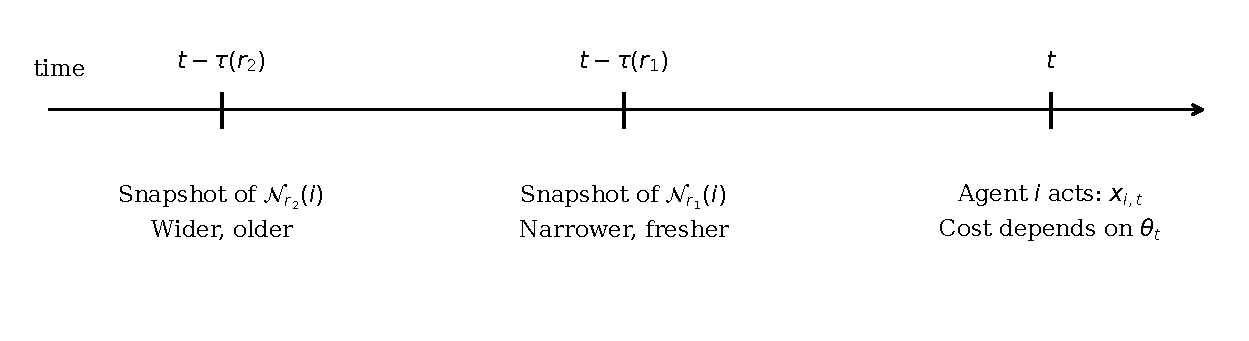
\includegraphics[width=\linewidth]{figures/snapshot_timing.pdf}
\caption{A radius-$r$ synchronized snapshot is taken at time $t-\tau(r)$ and
used for the decision at time $t$. For $r_2>r_1$ with $\tau(r_2)>\tau(r_1)$,
the wider snapshot is older. Cost is evaluated against the current state $\theta_t$.}
\label{fig:snapshot-timing}
\end{figure}
\begin{table}[htbp]
\centering\small
\setlength{\tabcolsep}{3pt}
\caption{Assumptions used in the derivations. All rows use square-integrable
targets and a deterministic positive-definite quadratic cost; normalized shares
require $R_\infty>0$. Entries describe the sufficient assumptions used by the
proofs, including their stated non-Gaussian extensions. ``Fixed epoch'' means
stationarity is unnecessary for that result.}
\label{tab:result-assumptions}
\begin{tabular}{@{}>{\raggedright\arraybackslash}p{.23\linewidth}>{\raggedright\arraybackslash}p{.12\linewidth}>{\raggedright\arraybackslash}p{.13\linewidth}>{\centering\arraybackslash}p{.095\linewidth}>{\centering\arraybackslash}p{.085\linewidth}>{\raggedright\arraybackslash}p{.275\linewidth}@{}}
\toprule
Result & Stationarity & Common-rate innovation & Affine target & Gaussian & Other \\
\midrule
Lemma~\ref{lem:radner_projection}; observation~\eqref{eq:general_crossover}
 & Fixed epoch & No & No & No & Admissible linear policy space \\
Lemma~\ref{lem:innovation_split}; Theorems~\ref{thm:OU_stale_regret}--\ref{thm:local_global_crossover}
 & Time & Yes & Yes & No & Scalar decay; finite-delay crossover as stated \\
Proposition~\ref{prop:aggregate_local}
 & Fixed epoch & No & Yes & No & Independent, mean-zero, equal-variance states \\
Threshold~\eqref{eq:aggregate_rho_star}
 & Time & Yes & Yes & No & Aggregate model plus temporal law \\
Theorem~\ref{thm:spatiotemporal_composition}
 & Time & Yes & Yes & No & Synchronized snapshots \\
Proposition~\ref{thm:marginal_balance}
 & Time & Yes & Yes & No & Differentiable $\tau,\eta_S$; $\eta_S<1$ \\
Lemma~\ref{prop:canonical_eta_S}
 & Space & No & Yes & Yes & $Q=qI$; exponential spatial covariance and kernel \\
Theorem~\ref{thm:canonical_optimal_radius}
 & Space/time & Yes & Yes & Yes & Canonical model and linear delay \\
\bottomrule
\end{tabular}
\end{table}

\clearpage
\section{Marginal-rate illustration}
Figure~\ref{fig:marginal-balance} illustrates how the marginal rates determine the optimal radius for the
canonical model in the main paper.
\begin{figure}[htbp]
\centering
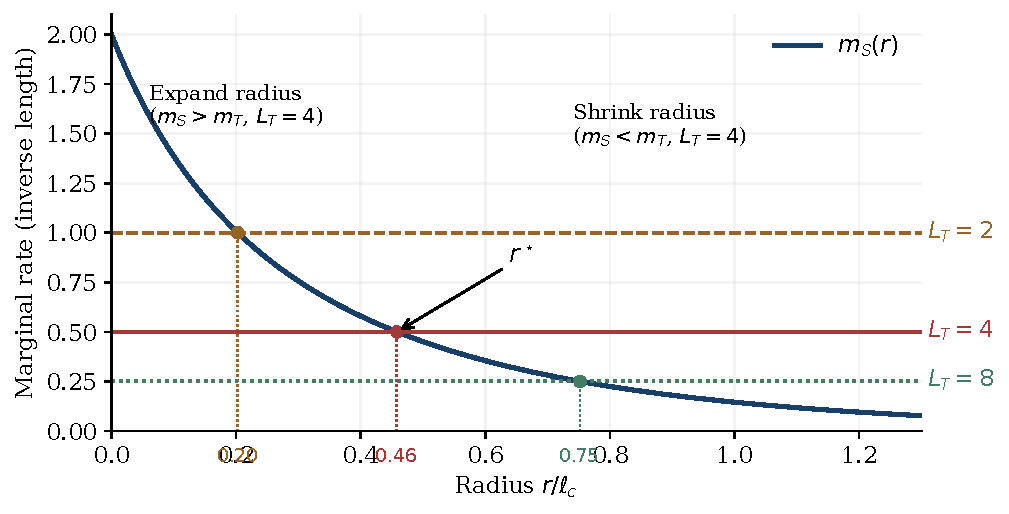
\includegraphics[width=.92\linewidth]{figures/marginal_balance.pdf}
\caption{Marginal balance in the canonical model with $\ell_c=1$ and
$\ell_s=0.5$. Increasing $L_T=vT$ lowers $m_T=2/L_T$ and moves the crossing
with $m_S$ outward. For the middle curve ($L_T=4$), regret falls to the left
of the crossing and rises to its right. This is an illustration of the
analytical rates, not an additional numerical experiment.}
\label{fig:marginal-balance}
\end{figure}
